\section{The Lossy Coherence Protocol}

\begin{figure}[t]
    \centerline{\includegraphics[scale=0.5]{figures/state_transition.pdf}}
    \caption{A Lossy Coherence with \storea implemented into a baseline MOESI Protocol.}
\label{fig:protocol}
\end{figure}




\begin{table}[t]
\caption{Coherence State Description for MOESI.}
\begin{tabular}{|ll|}
\hline
\textbf{State} & \textbf{Description} \\ \hline
\textbf{M}     &  \makecell[l]{Cache line is held exclusively by node\\ and is potentially dirty.}  \\ \hline
\textbf{O}     &  \makecell[l]{Cache line is owned by node and \\not held exclusively by others node.\\ Sharers may exist and is clean}\\ \hline
\textbf{E}     &  \makecell[l]{Cache line is held exclusively by node and is clean.}\\ \hline
\textbf{S}     &\makecell[l]{Cachle line is shared with 1 or more nodes and is clean.}\\ \hline
\textbf{I}    &\makecell[l]{Cache line is invalid.}\\ \hline
\end{tabular}
\label{tab:states}
\end{table}




\begin{figure}[t]
    \centering
    \begin{subfigure}[t]{0.5\textwidth}

        \centering
        \includegraphics[scale=0.5]{figures/transition_example.pdf}
        \caption{Baseline transition}
        \label{fig:base_transition}

    \end{subfigure}%

    \begin{subfigure}[t]{0.5\textwidth}
       
        \centering
        \includegraphics[scale=0.5]{figures/transition_approx_example.pdf}
        \caption{Lossy Coherence transition}
        \label{fig:lossy_transition}

    \end{subfigure}
\caption{Example coherence state transitions and requests for (a) baseline store, (b) Lossy Coherence \storea, to the I/S states }
\label{fig:transition}
\end{figure}

Lossy Coherence aims to exploit the high value locality of computation data store values to minimize coherence induced cache misses. This protocol extention targets approximate applications with tolerance to variations in output quality and introduces approximate stores (\storea) for data structures defined by the programmer. In this work, we demonstrate Lossy Coherence by extending a baseline (but not limited to) MOESI protocol.

\subsection{Approximate Stores}

Figure. \ref{fig:protocol} shows the addition of \storea instructions in a baseline MOESI protocol, and Table. \ref{tab:states} describes the coherence states. Stores to approximateable data structures are converted first into \storea. The \storea instructions can bypass coherence permission to write to blocks in invalid (I) and read-only states (S and O) whereas conventional stores would result in a miss. As long as the block's tag is present irrespective of coherence state, an \storea is able to write data. These \storea instructions reduce energy conspumption and latency within the memory heirachy by mitigating coherence traffic and data transfers. This is demonstrated in an example seen in Figure \ref{fig:transition}. Figure \ref{fig:transition}\subref{fig:base_transition} shows a possible set of coherence transactions upon a store to the L1 cache in the baseline MOESI directory protocol. The store would complete in 3 hops by, (1) sending GetX request to the L2 cache, (2) L2 sending invalidate requests to all sharers and responding to the requestor with data, (3) the sharers responding to the requestor with invalidation acknowledgements (Inv-Ack). Subsequest accesses to the invalidated blocks in the sharers would result in misses and hence further coherence transactions. In the Lossy protocol seen in Figure \ref{fig:transition}\subref{fig:lossy_transition}, if the store is an \storea, the write would be statisfied immediately, elimating the coherence transactions and state transitions saving both latency and energy. Subsequent access the blocks held by the sharers can still result in hits depending if its a load or store, although it may be accessing stale data. 

\storea instructions do not set the block's dirty-bit after modifing the data. Successive approximate stores to a clean block will maintain the block as clean until a normal store writes to it. Any approximate stores that follows a normal store will maintain the block as dirty. Advantages to treating \storea writes as clean is that it (1) requires less modification to the baseline protocol, and (2) reduces interconnection network bandwidth when silent evictions of clean blocks are supported.

\subsection{Programmer Annotations}

Stores are coverted to \storea on approximateable data structures which are annotated by the programmer by specifying the start and end addresses of the structure/structures. We only approximate data structures that store data used for compute. These structures may yield the most benefit if they are in frequently visited portions of code (e.g., values being updated in long loops). We do not approximate structures used for control flow, or ones that store memory addresses/pointers as it may cause undefined execution of the application and crash. The level of approximation within an application can be controlled by the programmer. If known beforehand, approximateable data structures that have poor approximate value locality can be omitted from approximation to reduce the amount of output error.

\subsection{Minimizing Output Error}


The Lossy protocol will effect the output accuracy of the application depending its inherent error-tolerance and the amount of \storea instructions. In circumstances where there may be many consecutive \storea to a value (e.g, incrementing a approximate data structure by 1 in a loop), we may want a method to prevent the value from becoming too divergent from its copies in other caches. We solve this by limiting the number of consecutive \storea to a fixed number $N$. For every $N^{th}$ \storea, the processor forces it to be a normal store so typical coherence transactions can take place, i.e., sending GetX and invalidating remote copies on the $N^{th}$ \storea. The $N-1$ \storea instructions accessing invalid or read-only blocks would recieve exclusive permission on the $N^{th}$ \storea (after forcing it to be a conventional store) and possibly coherent data. The $N-1$ \storea instructions already accessing exclusive data would set the block to dirty (if not already) on the $N^{th}$ \storea and update the copies in remote caches upon a writeback or data transfer. We can vary $N$ to change the level of approximation for each application. Values for $N$ would depend on application the level of accuracy needed. Higher values for $N$ would give \storea longer access to stale data, potenitally increasing performance by sacrificing output accuracy.


